%!TEX root = ../../THESIS.tex

\section{Drawing \& reading} \label{section:drawing}

The previous section defined diagrams as a data structure based on lists of layers, in this section we define \emph{pictures of diagrams}.
Concretely, such a picture will be encoded in a computer memory as a bitmap, i.e. a matrix of colour values.
Abstractly, we will define these pictures in terms of topological subsets of the Cartesian plane.
We first recall the topological definition from Joyal's and Street's unpublished manuscript \emph{Planar diagrams and tensor algebra}~\cite{JoyalStreet88} and then discuss the isomorphism between the two definitions.
In one direction, the isomorphism sends a \py{Diagram} object to its drawing.
In the other direction, it reads the picture of a diagram and translates it into a \py{Diagram} object, i.e. its domain, codomain and list of layers.

\subsection{Labeled generic progressive plane graphs}

A \emph{topological graph}, also called 1-dimensional cell complex, is a tuple $(G, G_0, G_1)$ of a Hausdorff space $G$ and a pair of a closed subset $G_0 \sub G$ and a set of open subsets $G_1 \sub P(G)$ called \emph{nodes} and \emph{wires} respectively, such that:
\begin{itemize}
\item $G_0$ is discrete and $G - G_0 = \bigcup G_1$,
\item each wire $e \in G_1$ is homeomorphic to an open interval and its boundary is contained in the nodes $\partial e \sub G_0$.
\end{itemize}
From a topological graph $G$, one can construct an undirected graph in the usual sense by forgetting the space $G$, taking $G_0$ as nodes and edges $(x, y) \in G_0 \times G_0$ for each $e \in G_1$ with $\partial e = \{ x, y \}$.
A topological graph is finite (planar) if its undirected graph is finite (planar, i.e. there is some embedding in the plane).

A \emph{plane graph} between two real numbers $a < b$ is a finite, planar topological graph $G$ with an embedding in $\R \times [a, b]$.
We define the domain $\dom(G) = G_0 \ \cap \ \R \times \{ a \}$, the codomain $\cod(G) = G_0 \ \cap \ \R \times \{ b \}$ as lists of nodes ordered by horizontal coordinates and the set $\boxes(G) = G_0 \ \cap \ \R \times (a, b)$.
We require that:
\begin{itemize}
    \item $G \ \cap \ \R \times \{ a \} = \dom(G)$ and $G \ \cap \ \R \times \{ b \} = \cod(G)$, i.e. the graph touches the horizontal boundaries only at domain and codomain nodes,
    \item every domain and codomain node $x \in G \ \cap \ \R \times \{ a, b \}$ is in the boundary of exactly one wire $e \in G_1$, i.e. wires can only meet at box nodes.
\end{itemize}
A plane graph is \emph{generic} when the projection on the vertical axis $p_1 : \R \times \R \to \R$ is injective on $G_0 \ - \ \R \times \{ a, b \}$, i.e. no two box nodes are at the same height.
From a generic plane graph, we can get a list $\boxes(G) \in G_0^\star$ ordered by height.
A plane graph is \emph{progressive} (also called \emph{recumbent} by Joyal and Street) when $p_1$ is injective on each wire $e \in G_1$, i.e. wires go from top to bottom and do not bend backwards.

From a progressive plane graph $G$, one can construct a directed graph by forgetting the space $G$, taking $G_0$ as nodes and edges $(x, y) \in G_0 \times G_0$ for each $e \in G_1$ with $\partial e = \{ x, y \}$ and $p_1(x) < p_1(y)$.
We can also define the domain and the codomain of each box node $\dom, \cod : \boxes(G) \to G_1^\star$ with
$\dom(x) = \{ e \in G_1 \ \vert \partial e = \{ x, y \}, p_1(x) < p_1(y) \}$ the wires coming in from the top and
$\cod(x) = \{ e \in G_1 \ \vert \partial e = \{ x, y \}, p_1(x) > p_1(y) \}$ the wires going out to the bottom, these sets are linearly ordered as follows.
Take some $\epsilon > 0$ such that the horizontal line at height $p_1(x) - \epsilon$ crosses each of the wires in the domain.
Then list $\dom(x) \in G_1^\star$ in order of horizontal coordinates of their intersection points, i.e. $e < e'$ if $p_0(y) < p_0(y')$ for the projection $p_0 : \R \times \R \to \R$ and $y^{(')} = e^{(')} \cap \{ p_1(x) - \epsilon \} \times \R$. Symmetrically we define the list of codomain nodes $\cod(x) \in G_1^\star$ with a horizontal line at $p_1 + \epsilon$.

A \emph{labeling} of progressive plane graph $G$ by a monoidal signature $\Sigma$ is a pair of functions from wires to objects $\lambda : G_1 \to \Sigma_0$ and from boxes to boxes $\lambda : \boxes(G) \to \Sigma_1$ which commutes with the domain and codomain.
From an lgpp (\emph{labeled generic progressive plane}) graph, one can construct a \py{Diagram}.

\begin{python}\label{listing:lgpp2diagram}
{\normalfont Reading a labeled generic progressive plane graphs as a \py{Diagram}.}
\vspace{5pt}
\hrule
\vspace{-15pt}
\begin{flalign*}
\py{def} \s & \py{read(} \s G, \s \lambda : G_1 \to \py{Ty}, \s \lambda : \boxes(G) \to \py{Box} \s \py{) -> Diagram:}&&\\
& \py{dom = [} \s \lambda(e) \s \py{for} \s x \in \dom(G) \s \py{for} \s e \in G_1 \s \py{if} \s x \in \partial e \s \py{]}&&\\
& \py{boxes = [} \s \lambda(x) \s \py{for} \s x \in \boxes(G) \s \py{]}&&\\
& \py{offsets = [len(} \s G_1 \ \cap \ \{ p_0(x) \} \times \R \s \py{) for} \s x \in \boxes(G) \s \py{]}&&\\
& \py{return decode(dom, zip(boxes, offsets))} &&
\vspace{-10pt}
\end{flalign*}
\hrule
\end{python}

\subsection{From diagrams to graphs and back}

In the other direction, there are many possible ways to draw a given \py{Diagram} as a lgpp graph, i.e. to embed its graph into the plane.
Vicary and Delpeuch \cite{VicaryDelpeuch22} give a linear-time algorithm to compute such an embedding with the following disadvantage: the drawing of a tensor $f \otimes g$ does not necessarily look like the horizontal juxtaposition of the drawings for $f$ and $g$.
For example, if we tensor an identity with a scalar, the wire representing the identity will wiggle around the node representing the scalar.
DisCoPy uses a quadratic-time drawing algorithm with the following design decision: we make every wire a straight line and as vertical as possible.
We first initialise the lgpp graph of the identity with a constant spacing between each wire, then for each layer we update the embedding so that there is enough space for the output wires of the box before we add it to the graph.
The resulting plane graph is then either plotted on the screen using Matplotlib~\cite{Hunter07} or translated to TikZ~\cite{Tantau13} code that can be integrated to a \LaTeX \ document.
All the diagrams in this thesis were drawn using DisCoPy together with TikZiT\footnote{\url{https://tikzit.github.io}} for manual editing.

\begin{python}
{\normalfont Outline of \py{Diagram.draw} from \py{Diagram} to \py{PlaneGraph}.}

\begin{minted}{python}
Embedding = dict[Node, tuple[float, float]]
PlaneGraph = tuple[Graph, Embedding]

def make_space(position: Embedding, scan: list[Node], box: Box, offset: int
        ) -> tuple[Embedding, float]:
    """ Update the graph to make space and return the left of the box. """

def draw(self: Diagram) -> PlaneGraph:
    graph = diagram2graph(self)
    box_nodes = [Node('box', box, -1, j) for j, box in enumerate(self.boxes)]
    dom_nodes = scan = [Node('dom', x, i, -1) for i, x in enumerate(self.dom)]
    position = {node: (i, -1) for i, node in enumerate(dom_nodes)}
    for j, (left, box, _) in enumerate(self.inside):
        box_node = Node('box', box, -1, j)
        position, left_of_box = make_space(position, scan, box, len(left))
        position[box_node] = (
            left_of_box + max(len(box.dom), len(box.cod)) / 2, j)
        for i, x in enumerate(box.dom):
            cod_node, = filter(lambda node: node.kind != "box",
                               graph.neighbors(Node('dom', x, i, j)))
            position[Node('dom', x, i, j)] = (position[cod_node][0], j - .1)
        for i, x in enumerate(box.cod):
            position[Node('cod', x, i, j)] = (left_of_box + i, j + .1)
        box_cod_nodes = [Node('cod', x, i, j) for i, x in enumerate(box.cod)]
        scan = scan[:len(left)] + box_cod_nodes + scan[len(left @ box.dom):]
    for i, x in enumerate(self.cod):
        cod_node = Node('cod', x, i, len(self))
        position[cod_node] = (position[scan[i]][0], len(self))
    return graph, position

Diagram.draw = draw
\end{minted}
\end{python}

Note that when we draw the plane graph for a diagram, we do not usually draw the box nodes as points.
Instead, we draw them as boxes, i.e. a box node $x \in \boxes(G)$ is depicted as the rectangle with corners $(l, p_1(x) \pm \epsilon)$ and $(r, p_1(x) \pm \epsilon)$ for $l, r \in \R$ the left- and right-most coordinate of its domain and codomain nodes.
In this way, we do not need to draw the in- and out-going wires of the box node: they are hidden by the rectangle.
Exceptions include \emph{spider boxes} where we draw the box node (the head) and its outgoing wires (the legs of the spider) as well as \emph{swap, cup and cap boxes} where we do not draw the box node at all, only its outgoing wires which are drawn as Bézier curves to look like swaps, cups and caps respectively.
These special boxes will be discussed, and drawn, in section~\ref{section:extra structure}.

\begin{example}
{\normalfont Drawing of a box, an identity, a layer, a composition and a tensor.}

\begin{minted}{python}
a, b, c, x, y, z, w = map(Ty, "abcxyzw")
Box('box', a @ b, x @ y @ z).draw()
\end{minted}

\ctikzfig{img/basics/box}

\begin{minted}{python}
Diagram.id(x @ y @ z).draw()
\end{minted}

\ctikzfig{img/basics/id}

\begin{minted}{python}
layer = a @ Box('f', x, y) @ b
layer.draw()
\end{minted}

\ctikzfig{img/basics/layer}

\begin{minted}{python}
top, bottom = Box('top', a @ b, x @ y @ z), Box('bottom', x @ y @ z, c)
(top >> bottom).draw()
\end{minted}

\ctikzfig{img/basics/composition}

\begin{minted}{python}
left, right = Box('left', a @ b, x @ y @ z), Box('right', x @ y @ z, c)
(left @ right).draw()
\end{minted}

\ctikzfig{img/basics/tensor}
\end{example}

\begin{example}
{\normalfont Drawing of the interchanger in the general case.}

\begin{minted}{python}
f, g = Box('f', x, y), Box('g', z, w)
(a @ f @ b @ g @ c).interchange(0).draw(); (a @ f @ b @ g @ c).draw()
\end{minted}

\begin{center}
\tikzfig{img/basics/interchanger-left}
$\quad \to_R \quad$ \tikzfig{img/basics/interchanger-right}
\end{center}
\end{example}

\begin{example}
{\normalfont Drawing of the interchangers for an effect then a state.}

\begin{minted}{python}
f, g = Box('f', x, Ty()), Box('g', Ty(), w)
(f >> g).interchange(0).draw()
(f >> g).draw()
(f >> g).interchange(0, left=True).draw()
\end{minted}

\begin{center}
\tikzfig{img/basics/state-effect-left}
$\quad \to_R \quad$ \tikzfig{img/basics/state-effect}
$\quad \to_R \quad$ \tikzfig{img/basics/state-effect-right}
\end{center}
\end{example}

\begin{example}
{\normalfont Drawing of the Eckmann-Hilton argument.}

\begin{minted}{python}
f, g = Box('f', Ty(), Ty()), Box('g', Ty(), Ty())
(f @ g).draw()
(f @ g).interchange(0).draw()
(f @ g).interchange(0).interchange(0).draw()
\end{minted}

\begin{center}
\tikzfig{img/basics/Eckmann-Hilton-left}
$\quad \to_R \quad$ \tikzfig{img/basics/Eckmann-Hilton-right}
$\quad \to_R \quad$ \tikzfig{img/basics/Eckmann-Hilton-left}
$\quad \to_R \quad \dots$
\end{center}
\end{example}

\begin{example}\label{example:spiral}
The following spiral diagram is the cubic worst-case for interchanger normal form.
It is also the quadratic worst-case for drawing, at each layer of the first half we need to update the position of every preceding layer in order to make space for the output wires.

\begin{minted}{python}
x = Ty('x')
f, g = Box('f', Ty(), x @ x), Box('g', x @ x, Ty())
u, v = Box('u', Ty(), x), Box('v', x, Ty())

def spiral(length: int) -> Diagram:
    diagram, n = u, length // 2 - 1
    for i in range(n):
        diagram >>= x ** i @ f @ x ** (i + 1)
    diagram >>= x ** n @ v @ x ** n
    for i in range(n):
        diagram >>= x ** (n - i - 1) @ g @ x ** (n - i - 1)
    return diagram

diagram = spiral(8)
for i in [1, 2, 3]: diagram[:i + 1].draw()
diagram.draw(); diagram.normal_form().draw()
Diagram.to_gif(*diagram.normalize())
\end{minted}
\begin{center}
\tikzfig{img/spiral/1},
\tikzfig{img/spiral/2},
\tikzfig{img/spiral/3}, ... \\
\vspace{5pt}
\tikzfig{img/spiral/8} $\quad \sim \quad$
\tikzfig{img/spiral/nf}
\end{center}
The interchangers between these two diagrams can be downloaded as a \py{.gif}\footnote
{\href{https://github.com/oxford-quantum-group/discopy/blob/f364ce218890d87fda4aa5c1f4f770f07c7b4f25/docs/_static/imgs/spiral.gif}{\nolinkurl{https://github.com/oxford-quantum-group/discopy/.../imgs/spiral.gif}}} video.
\end{example}

Next, we define the inverse translation \py{graph2diagram}.
\pagebreak

\begin{python}\label{listing:graph2diagram}
{\normalfont Translation from \py{PlaneGraph} to \py{Diagram}.}

\begin{minted}{python}
def graph2diagram(graph: Graph, position: Embedding) -> Diagram:
    dom = Ty(*[node.label for node in graph.nodes
               if node.kind == 'dom' and node.j == -1])
    boxes = [node.label for node in graph.nodes if node.kind == 'box']
    scan, offsets = [Node('dom', x, i, -1) for i, x in enumerate(dom)], []
    for j, box in enumerate(boxes):
        left_of_box = position[Node('dom', box.dom[0], 0, j)][0]\
            if box.dom else position[Node('box', box, -1, j)][0]
        offset = len([node for node in scan if position[node][0] < left_of_box])
        box_cod_nodes = [Node('cod', x, i, j) for i, x in enumerate(box.cod)]
        scan = scan[:offset] + box_cod_nodes + scan[offset + len(box.dom):]
        offsets.append(offset)
    return decode(Encoding(dom, list(zip(boxes, offsets))))
\end{minted}
\end{python}

\begin{proposition}\label{proposition:graph2diagram(self.draw())}
The equality \py{graph2diagram(self.draw()) == self} holds for all \py{self: Diagram}.
\end{proposition}

\begin{proof}
By induction on \py{n = len(self)}.
If \py{n == 0} we get that \py{dom == self.dom} and \py{boxes == offsets == []}.
If the proposition holds for \py{self}, then it holds for \py{self} \py{>> Layer(left, box, right)}.
Indeed, we have:
\begin{itemize}
\item \py{dom == self.dom and boxes == self.boxes + [box]}
\item \py{(x, Node('cod', self.cod[i], i, n)) in graph}\\
\noindent \py{for i, x in enumerate(scan)}
\end{itemize}
Moreover, the horizontal coordinates of the nodes in \py{scan} are strictly increasing,
thus we get the desired \py{offsets == self.offsets + [len(left)]}.
\end{proof}

From a labeled generic progressive plane graph, we get a unique diagram \emph{up to deformation}.
A deformation $h : G \to G'$ between two labeled plane graphs $G, G'$ is a continuous map $h : G \times [0, 1] \to \R \times \R$ such that:
\begin{itemize}
\item $h(G, t)$ is a plane graph for all $t \in [0, 1]$, $h(G, 0) = G$ and $h(G, 1) = G'$,
\item $x \in \boxes(G)$ implies $h(x, t) \in \boxes(h(G, t))$ for all $t \in [0, 1]$,
\item $h(G, t) \fcmp \lambda = \lambda$ for all $t \in [0, 1]$, i.e. the labels are preserved throughout.
\end{itemize}
A deformation is progressive (generic) when $h(G, t)$ is progressive (generic) for all $t \in [0, 1]$.
We write $G \sim G'$ when there exists some deformation $h : G \to G'$, this defines an equivalence relation.

\begin{proposition}\label{proposition:g2d then d2g}
\py{Diagram.draw(graph2diagram(} $G$ \py{))} $\sim G$ for all lgpp graphs $G$, up to generic progressive deformation.
\end{proposition}

\begin{proof}
By induction on the length of $\boxes(G)$.
If there are no boxes, $G$ is the graph of the identity and we can deform it so that each wire is vertical with constant spacing.
If there is one box, $G$ is the graph of a layer and we can cut it in three vertical slices with the box node and its outgoing wires in the middle.
We can apply the case of the identity to the left and right slices, for the middle slice we make the wires straight with a constant spacing between the domain and codomain.
Because $G$ is generic, we can cut a graph with $n > 2$ boxes in two horizontal slices between the last and the one-before-last box, then apply the case for layers and the induction hypothesis.
To glue the two slices back together while keeping the wires straight, we need to make space for the wires going out of the box.

This deformation is indeed progressive, i.e. we never bend wires, we only make them straight.
It is also generic, i.e. we never move a box node past another.
\end{proof}

\begin{proposition}\label{proposition:d2g then g2d}
There is a progressive deformation $h : G \to G'$ between two lgpp graphs iff \py{graph2diagram(} $G$ \py{) == graph2diagram(} $G'$ \py{)} up to interchanger.
\end{proposition}

\begin{proof}
By induction on the number $n$ of \emph{coincidences}, the times at which the deformation $h$ fails to be generic, i.e. two or more boxes are at the same height.
WLOG (i.e. up to continuous deformation of deformations) this happens at a discrete number of time steps $t_1, \dots, t_n \in [0, 1]$.
Again WLOG at each time step there is at most two boxes at the same height, e.g. if there are two boxes moving below a third at the same time, we deform the deformation so that they move one after the other.
The list of boxes and offsets is preserved under generic deformation, thus if $n = 0$ then \py{graph2diagram(} $G$ \py{) == graph2diagram(} $G'$ \py{)} on the nose.
If $n = 1$, take \py{i: int} the index of the box for which the coincidence happens and \py{left: bool} whether it is a left or right interchanger, then \py{graph2diagram(} $G$ \py{).interchange(i, left) == graph2diagram(} $G'$ \py{)}.
Given a deformation with $n + 1$ coincidences, we can cut it in two time slices with $1$ and $n$ coincidences respectively then apply the cases for $n = 1$ and the induction hypothesis.

For the converse, a proof of \py{graph2diagram(} $G$ \py{) == graph2diagram(} $G'$ \py{)}, i.e. a sequence of $n$ interchangers, translates into a deformation with $n$ coincidences.
DisCoPy can output these proofs as videos using \py{Diagram.normalize} to iterate through the rewriting steps and \py{Diagram.to_gif} to produce a \py{.gif} file.
\end{proof}

\subsection{A natural isomorphism}

We have established an isomorphism between the class of lgpp graphs (up to progressive deformation) and the class of \py{Diagram} objects (up to interchanger).
It remains to define lgpp graphs as the arrows of a monoidal category, i.e. to define identity, composition and tensor.
For every monoidal signature $\Sigma$, there is a monoidal category $G(\Sigma)$ with objects $\Sigma_0^\star$ and arrows the equivalence classes of lgpp graphs with labels in $\Sigma$.
The domain and codomain of an arrow is given by the labels of the domain and codomain of the graph.
The identity $\id(x_1 \dots x_n)$ is the graph with wires $(i, a) \to (i, b)$ for $i \leq n$ and $a, b \in \R$ the horizontal boundaries.
The tensor of two graphs $G$ and $G'$ is given by horizontal juxtaposition, i.e. take $w = \max(p_0(G)) + 1$ the right-most point of $G$ plus a margin and set $G \otimes G' = G \cup \{ (p_0(x) + w, p_1(x)) \ \vert \ x \in G' \}$.
The composition $G \fcmp G'$ is given by vertical juxtaposition and connecting the codomain nodes of $G$ to the domain nodes of $G'$.
That is, $G \fcmp G' = s^+(G) \cup s^-(G') \cup E$ for $s^\pm(x) = \big( p_0(x), \frac{p_1(x) \pm (b - a)}{2} \big)$ and wires $s^+(\cod(G)_i) \to s^-(\dom(G')_i) \in E$ for each $i \leq \len(\cod(G)) = \len(\dom(G'))$.

The deformations for the unitality axioms are straightforward: there is a deformation $G \fcmp \id(\cod(G)) \sim G \sim \id(\dom(G)) \fcmp G$ which contracts the wires of the identity graph, the unit of the tensor is the empty diagram so we have an equality $G \otimes \id(1) = G = \id(1) \otimes G$.
The deformations for the associativity axioms are better described by the hand-drawn diagrams of Joyal and Street in figure~\ref{fig:assoc}.

\begin{figure}[H]
\centering
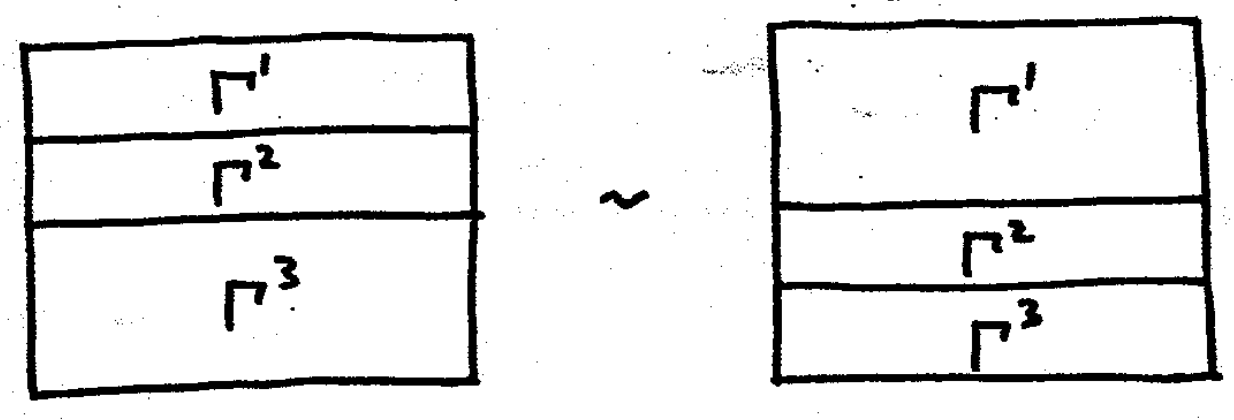
\includegraphics[scale=0.2]{img/tensor-assoc.png}
\qquad \quad 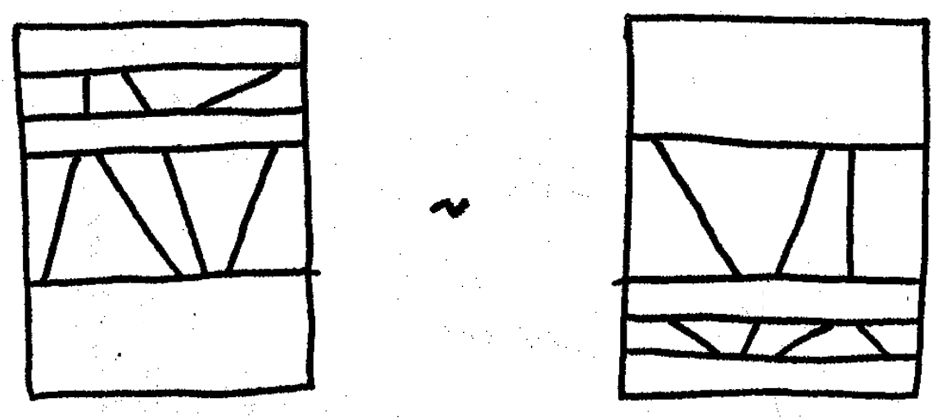
\includegraphics[scale=0.2]{img/compos-assoc.png}
\caption{Deformations for the associativity of tensor and composition.}
\label{fig:assoc}
\end{figure}

The interchange law holds on the nose, i.e. $(G \otimes G') \fcmp (H \otimes H') = (G \fcmp H) \otimes (G' \fcmp H')$, as witnessed by figure~\ref{fig:interchange}, the hand-drawn diagram which is the result of both sides.

\begin{figure}[H]
\centering
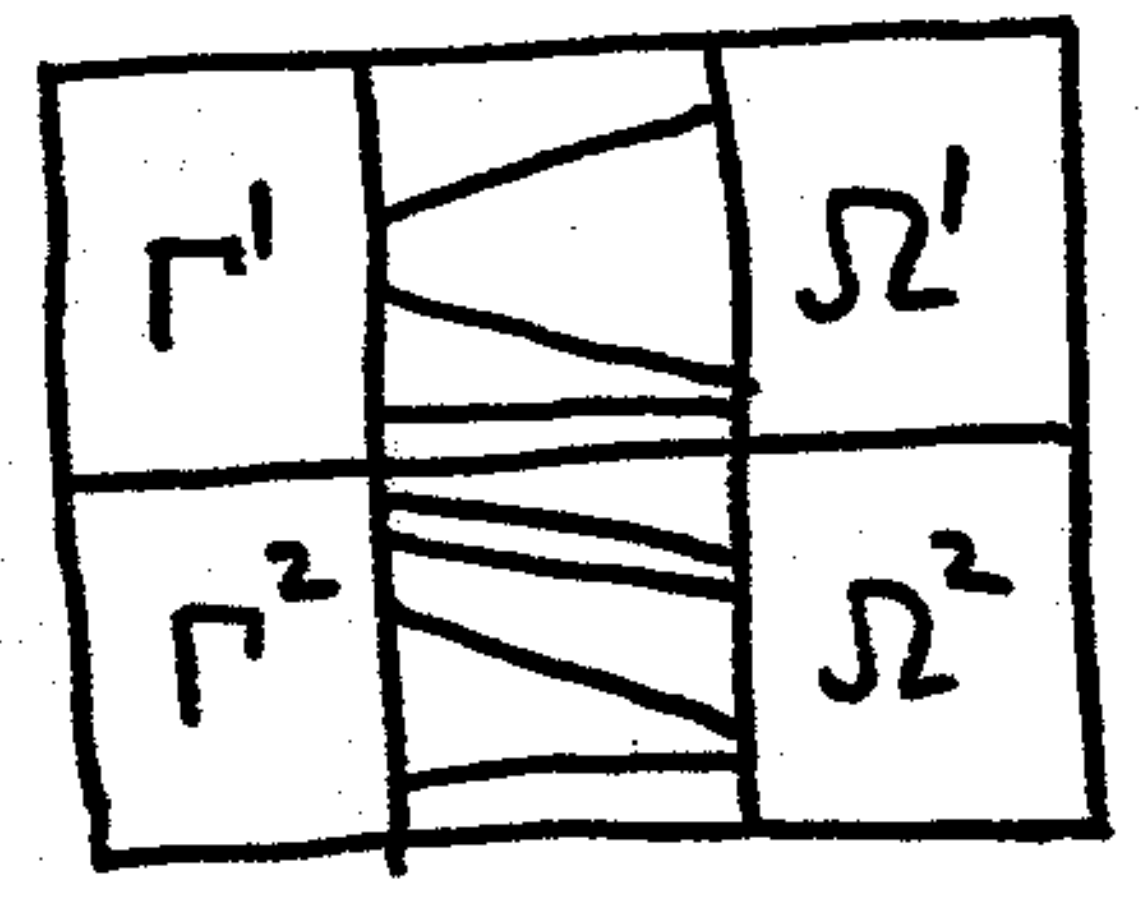
\includegraphics[scale=0.1]{img/interchange.png}
\caption{The graph of the interchange law.}
\label{fig:interchange}
\end{figure}

Thus, we have defined a monoidal category $G(\Sigma)$.
Now given a morphism of monoidal signatures $f : \Sigma \to \Sigma'$, we can define a functor $G(f) : G(\Sigma) \to G(\Sigma')$ which sends a graph to itself relabeled with $f \fcmp \lambda$, its image on arrows is given in listing~\ref{listing:G_of_f}.
Hence, we have defined a functor\footnote
{For lack of a better notation, we use the same letter $G$ to refer to an arbitrary graph as well as for the functor $G  : \mathbf{MonSig} \to \mathbf{MonCat}$.} $G : \mathbf{MonSig} \to \mathbf{MonCat}$ which we claim is naturally isomorphic to the free functor $F : \mathbf{MonSig} \to \mathbf{MonCat}$ defined in the previous section.
An abstract way to prove this is to appeal to the universal property of free monoidal categories: if the topological and the combinatorial definitions are both free monoidal, they are necessarily isomorphic.
More concretely, we can implement this natural isomorphism as a commutative diagram in $\mathbf{Pyth}$ and think of it as a software test for our drawing and reading algorithms.

\begin{python}\label{listing:G_of_f}
{\normalfont Implementation of the functor $G : \mathbf{MonSig} \to \mathbf{MonCat}$.}

\begin{minted}{python}
SigMorph = tuple[dict[Ob, Ob], dict[Box, Box]]

def G(f: SigMorph) -> Callable[[Graph], Graph]:
    def G_of_f(graph: Graph) -> Graph:
        relabel = lambda node: Node('box', f[1][node.label], node.i, node.j)\
            if node.kind == 'box'\
            else Node(node.kind, f[0][node.label], node.i, node.j)
        return Graph(map(relabel, graph.edges))
    return G_of_f
\end{minted}
\end{python}

\begin{proposition}\label{proposition:nat-iso}
There is a natural isomorphism $F \simeq G : \mathbf{MonSig} \to \mathbf{MonCat}$ for $F$ the combinatorial definition of diagrams in section~\ref{subsection:free-monoidal} and $G$ the topological definition in terms of labeled generic progressive plane graphs.
\end{proposition}

\begin{proof}
From propositions~\ref{proposition:g2d then d2g} and \ref{proposition:d2g then g2d}, we have an isomorphism between \py{Diagram} and \py{PlaneGraph} (up to deformation and interchanger respectively) given by \py{d2g = Diagram.draw} and \py{g2d = graph2diagram}.
Now define the image of $F$ on arrows \py{F = lambda f: Functor(ob=f[0], ar=f[1])}.
Given a morphism of monoidal signatures \py{f: SigMorph} we have the following two naturality squares.
\begin{center}
    \begin{tikzcd}
    \py{Diagram} \ar{r}{\py{d2g}} \ar{d}[']{\py{F(f)}} &
    \py{PlaneGraph} \ar{d}{\py{G(f)}}\\
    \py{Diagram} \ar{r}{\py{d2g}} &
    \py{PlaneGraph}
    \end{tikzcd}
    \qquad \text{and} \qquad
    \begin{tikzcd}
    \py{PlaneGraph} \ar{r}{\py{g2d}} \ar{d}[']{\py{G(f)}} &
    \py{Diagram} \ar{d}{\py{F(f)}}\\
    \py{PlaneGraph} \ar{r}{\py{g2d}} &
    \py{Diagram}
    \end{tikzcd}
\end{center}
\end{proof}

\subsection{Daggers, sums and bubbles}

As in the previous sections, we now discuss the drawing of daggers, sums and bubbles.
When we draw a diagram in the free $\dagger$-monoidal category, we add some asymmetry to the drawing of each box so that it looks like the vertical reflection of its dagger.

\begin{example}
{\normalfont Drawing of the axiom for unitaries.}

\begin{minted}{python}
f, g = Box('f', x, y), Box('g', z, w)
(f >> f[::-1]).draw(); Diagram.id(x).draw()
(f[::-1] >> f).draw(); Diagram.id(y).draw()
\end{minted}

\begin{center}
\tikzfig{img/basics/unitaries-left} \hspace{100pt}
\tikzfig{img/basics/unitaries-right}
\end{center}
\end{example}

\begin{example}
{\normalfont Drawing of the axiom for $\dagger$-monoidal categories.}

\begin{minted}{python}
f, g = Box('f', x, y), Box('g', z, w)
(f @ g)[::-1].draw(); (f[::-1] @ g[::-1]).draw()
assert (f @ g)[::-1].normal_form() == f[::-1] @ g[::-1]
\end{minted}

\begin{center}
\tikzfig{img/basics/dagger-monoidal-left}
$\quad \to_R \quad$ \tikzfig{img/basics/dagger-monoidal-right}
\end{center}
\end{example}

When we draw a sum, we just draw each term with an addition symbol in between.
More generally, \py{drawing.equation} allows to draw any list of diagrams and \py{drawing.Equation} allows to draw equations within equations.

\begin{example}
{\normalfont Drawing of a commutativity equation.}

\begin{minted}{python}
from discopy import drawing

f, g, h = Box('f', x, y), Box('g', y, z), Box('h', x, z)
drawing.equation(drawing.Equation(f >> g, h, symbol='$+$'),
                 drawing.Equation(h, f >> g, symbol='$+$'))
\end{minted}
\ctikzfig{img/basics/equation}
\end{example}

\begin{example}
{\normalfont Drawing a composition and tensor of sums.}

\begin{minted}{python}
f0, g0 = Box("f0", x, y), Box("g0", y, z)
f1, g1 = Box("f1", x, y), Box("g1", y, z)
((f0 + f1) >> (g0 + g1)).draw()
\end{minted}
\ctikzfig{img/basics/sums-composition}

\begin{minted}{python}
((f0 + f1) @ (g0 + g1)).draw()
\end{minted}
\ctikzfig{img/basics/sums-tensor}
\end{example}

The case of drawing bubbles is more interesting.
One solution would be to draw the bubble as a rectangle like any other box, then draw the content of the bubble inside the rectangle.
However, this would require some clever scaling so that the boxes of the diagram inside the bubble have the same size as the boxes outside, i.e. we would need to add more complexity to our drawing algorithm.
The solution implemented in DisCoPy is to apply a faithful functor $\py{downgrade} : F(\Sigma^\beta) \to F(\Sigma \cup \mathtt{open}^\beta \cup \mathtt{close}^\beta)$ from the free monoidal category with bubbles $F(\Sigma^\beta)$ to the free monoidal category generated by the following signature.
Take the objects $\mathtt{open}^\beta_0 = \mathtt{close}^\beta_0 = \Sigma_0 + \{ \bullet \}$ and boxes
for opening $\mathtt{open}^\beta(x) : \beta_\dom(x) \to \bullet \otimes x \otimes \bullet$ and closing $\mathtt{close}^\beta(x) : \bullet \otimes x \otimes \bullet \to \beta_\cod(x)$ bubbles for each type $x \in \Sigma_0^\star$.
Now define $\py{downgrade(f.bubble())} = \mathtt{open}^\beta(\py{f.dom}) \fcmp (\bullet \otimes \py{f} \otimes \bullet) \fcmp \mathtt{close}^\beta(\py{f.cod})$ for any diagram $\py{f}$ inside a bubble.
That is, we draw a bubble as its opening, its inside with identity wires on both sides then its closing.
The $\bullet$-labeled wires are drawn with Bézier curves so that the bubble looks a bit closer to a circle than a rectangle.
In the case of bubbles that are length-preserving on objects, we also want to override the drawing of its opening and closing boxes so that the wires go straight through the bubble rather than meeting at the box node.

\begin{example}
{\normalfont Drawing of a bubbled diagram and a first-order logic formula.}

\begin{minted}{python}
f, g, h = Box('f', x, y), Box('g', y, z), Box('h', y @ z, x)
(f @ g >> h).bubble(dom=a @ b, cod=c, name="$\\beta$").draw()
\end{minted}
\ctikzfig{img/basics/bubble}
\begin{minted}{python}
god = Predicate("G", x)
formula = god >> (Formula.id(x).cut() >> god.dagger()).cut()
formula.draw()
\end{minted}
\ctikzfig{img/basics/there-is-but-one-god}
\end{example}

\subsection{Automatic diagram recognition}

We conclude this section with an application of proposition~\ref{proposition:nat-iso} to \emph{automatic diagram recognition}: turning pictures of diagrams into diagrams.
In listing~\ref{listing:lgpp2diagram}, we described an abstract reading algorithm which took lgpp graphs as input and returned diagrams.
We make it a concrete algorithm by taking \emph{bitmaps} as input: grids of Boolean pixels describing a black-and-white picture.
The algorithm \py{read} listed below takes as input a pair of bitmaps for the box nodes and the wires of the plane graph, it returns a \py{Diagram}.
It is more general than the \py{graph2diagram} algorithm of listing~\ref{listing:lgpp2diagram} where we assumed that the embedding of the graph looked like the output of \py{Diagram.draw}. i.e. that edges are straight vertical lines.
Indeed, our reading algorithm will accept \emph{any bitmaps} as input and always return a valid diagram, however bended the edges are.
If the bitmaps indeed represent a progressive generic plane graph $G$, then we get \py{read(} $G$ \py{).draw()} $\sim G$ up to progressive generic deformation.
If not, the output will still be a diagram but its drawing may not look anything like the input.

\begin{python}
{\normalfont Implementation of the abstract reading algorithm of listing~\ref{listing:lgpp2diagram}.}

\begin{minted}{python}
from numpy import array, argmin
from skimage.measure import regionprops, label

def read(box_pixels: array, wire_pixels: array) -> Diagram:
    connected_components = lambda img: regionprops(label(img))
    box_nodes, wires = map(connected_components, (box_pixels, wire_pixels))
    source, target, length, width = [], [], len(box_pixels), len(box_pixels[0])
    critical_heights = [0] + [
        int(node.centroid[0]) for node in box_nodes] + [length]
    for wire, region in enumerate(wires):
        top, bottom = (
            minmax(i for i, _ in region.coords) for minmax in (min, max))
        source.append(argmin(abs(array(critical_heights) - top)))
        target.append(argmin(abs(array(critical_heights) - bottom)))
    scan = [wire for wire, node in enumerate(source) if node == 0]
    dom, boxes_and_offsets = Ty('x') ** len(scan), []
    for depth, box_node in enumerate(box_nodes):
        input_wires = [wire for wire in scan if target[wire] == depth + 1]
        output_wires = [
            wire for wire, node in enumerate(source) if node == depth + 1]
        dom, cod = Ty('x') ** len(input_wires), Ty('x') ** len(output_wires)
        box = Box('box_{}_{}'.format(len(dom), len(cod)), dom, cod)
        height, left = map(int, box_node.centroid)
        left_of_box = [wire for wire in scan if wire not in input_wires
                       and dict(wires[wire].coords).get(height, width) < left]
        offset = max(len(left_of_box), 0)
        boxes_and_offsets.append((box, offset))
        scan = scan[:offset] + output_wires + scan[offset + len(input_wires):]
    return decode(dom, tuple(boxes_and_offsets))
\end{minted}
\end{python}

We use the \py{array} data structure of NumPy~\cite{VanDerWaltEtAl11} for bitmaps.
We compute the connected components of box and wire pixels with Scikit-Image~\cite{WaltEtAl14}, using their default ordering by lexicographic order of top-left pixel.
We then define a list of critical heights: the top of the picture, the height of the centroid of each box component, then the bottom of the picture.
For each wire component, we define its source and target as the closest critical height to its top-most and bottom-most pixel.
We define the domain of the diagram as the list of wires with the domain as source.
We then scan through the picture top to bottom, keeping a list \py{scan} of the open wires at each height.
For each box, we find its input wires in this list and define the offset as the number of wires left of the box node that are not inputs, then we update \py{scan} with the output wires.
We get an encoding \py{dom, boxes_and_offsets} which yields a valid diagram by construction.

\begin{example}
Suppose we take the following picture of a diagram as input, where the red pixels are boxes and the black pixels are wires:
\begin{center}
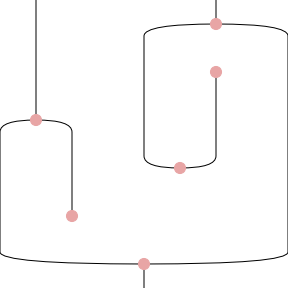
\includegraphics[scale=.2]{img/bitmap2diagram/start.png}
\end{center}
We count $\{ 1, \dots, 6 \}$ boxes and 8 wires
$$
\{ 0 \to 3, \s
0 \to 1, \s
1 \to 4, \s
1 \to 6, \s
2 \to 4, \s
3 \to 6, \s
3 \to 5, \s
6 \to 7 \}
$$
for $0$ and $7$ the domain and codomain of the whole diagram respectively.
\begin{center}
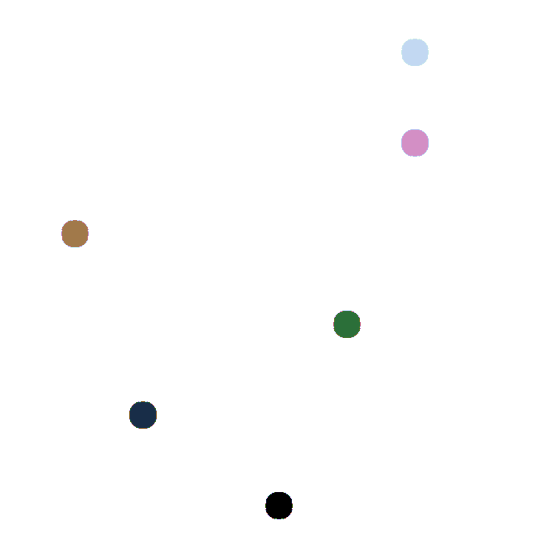
\includegraphics[scale=.2]{img/bitmap2diagram/boxes.png}
\hspace{10pt}
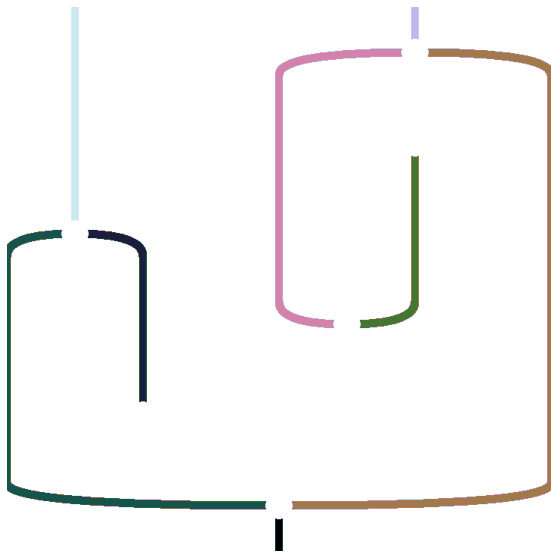
\includegraphics[scale=.2]{img/bitmap2diagram/wires.png}
\end{center}

From this, we reconstruct the following diagram by scanning top to bottom:

\ctikzfig{img/bitmap2diagram/finish}

which is indeed equal to the input picture, up to generic progressive deformation.
\end{example}

\begin{example}
Suppose we start from the following pastiche of Kandinsky's \emph{Punkt und linie zu fläche} (point and line on the plane):

\begin{center}
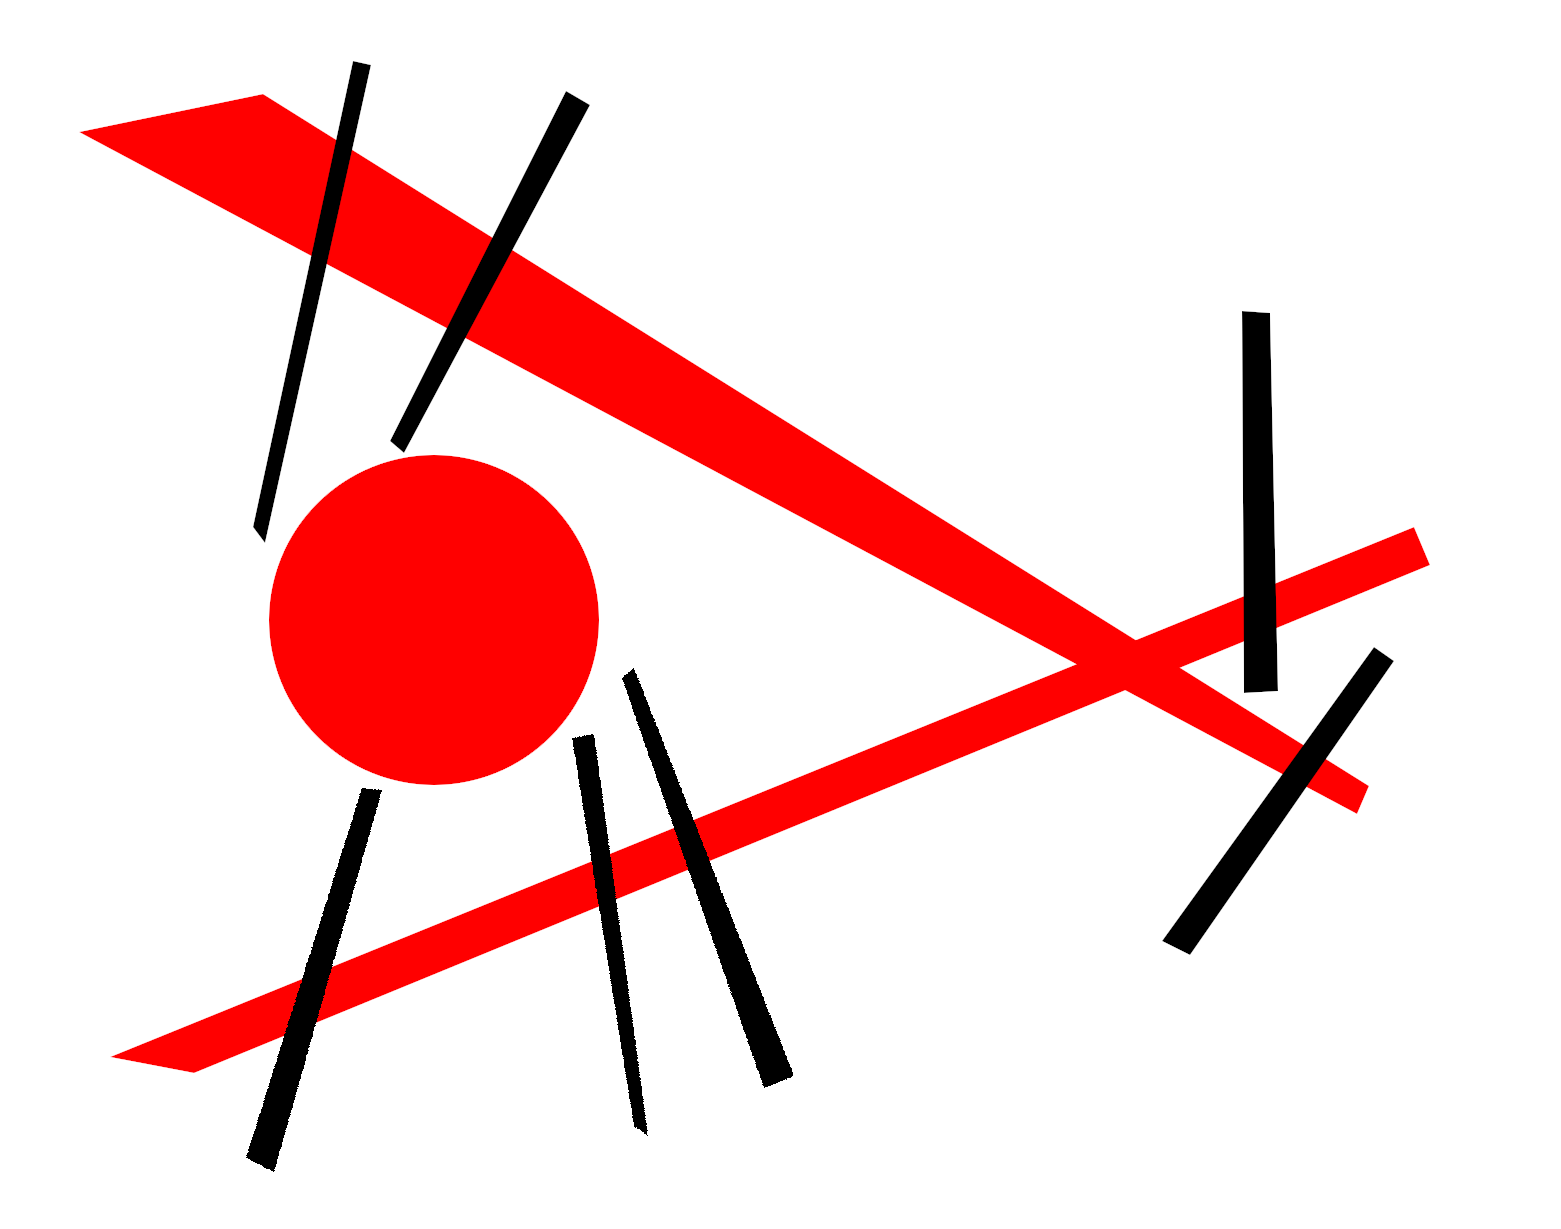
\includegraphics[scale=.4]{img/punkt-und-linie/start.png}
\end{center}
We count $\{ 1, \dots, 9 \}$ boxes and 7 wires
$$\{
0 \to 3, \s
1 \to 3, \s
2 \to 4, \s
4 \to 8, \s
4 \to 9, \s
6 \to 10, \s
6 \to 10 \}
$$
for $0$ and $10$ the domain and codomain of the whole diagram respectively.
\begin{center}
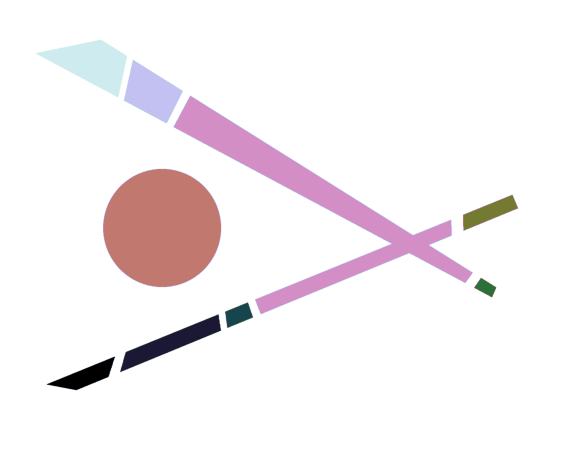
\includegraphics[scale=.2]{img/punkt-und-linie/boxes.png}
\hspace{10pt}
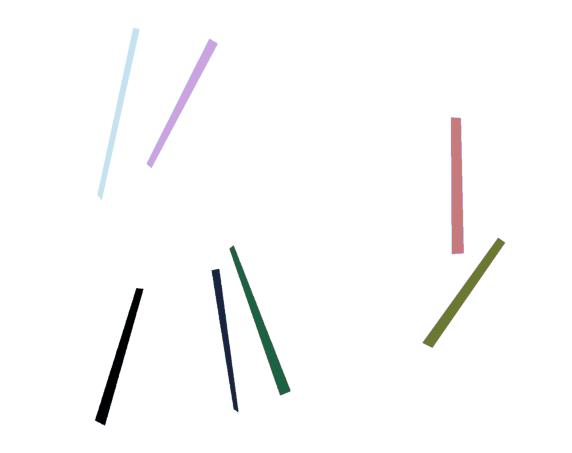
\includegraphics[scale=.2]{img/punkt-und-linie/wires.png}
\end{center}

From this, we reconstruct the following diagram by scanning top to bottom:

\ctikzfig{img/punkt-und-linie/finish}

which looks nothing like the input because Kandinsky's abstract paintings are not generic progressive plane graphs.
\end{example}

What could be the applications of such a reading algorithm?
Of course, real-world pictures do not come in clean red and black bitmaps.
We need some more computer vision to label each pixel as belonging either to a box, a wire or the background.
This can be achieved by training a convolutional neural network on a large number of example pictures, each annotated with their red and black bitmaps.
Once we have trained the machine to classify whether pixels belong to a box or wire, we can also train it to output the label of each pixel, i.e. the label of the box or wire it belongs to.
With enough training data, we could automatically turn pictures of Bob's blackboard into circuits that we can execute on a quantum computer.
Less trivially, this could be applied to \emph{document layout analysis}:
from the picture of say, a hand-drawn calendar from the middle ages, we could train our recognition algorithm to output a diagram that encodes the structure of the calendar.
In previous work~\cite{BorosEtAl19}, we trained convolutional neural networks to extract lines of text in medieval manuscripts, but we had to exclude calendars from our analysis due to the complexity of their layouts.
Our diagram recognition machines would enhance the automated analysis of such hand-drawn documents with structured layouts.

Our simple algorithm is robust to any deformation of lgpp graph, but there is much room for improvement.
The easiest assumption to remove is genericity, i.e. boxes need not be at distinct heights.
Non-generic progressive plane graphs, i.e. with potentially horizontal wires between boxes at the same height, have been characterised as the arrows of free \emph{double categories}.
Delpeuch~\cite{Delpeuch20} shows how they can be encoded as lgpp graphs with an extra label on each wire for whether it is horizontal or vertical.
We can also remove the progressivity assumption, i.e. wires can bend backwards.
We have two options: either a) we write a geometric algorithm than can find the endpoints of any bended wire, or b) we train another neural network to detect each point of non-progressivity, i.e. the cups and caps where the vertical derivative of a wire changes sign.
Such non-progressive plane graphs can be encoded as lgpp graphs with \emph{cups and caps boxes}, they are the arrows of free \emph{pivotal categories} which we discuss in section~\ref{subsection:rigid}.

Next, we can get rid of the planarity assumption: the projection of the topological graph onto the plane need not be an embedding, i.e. wires can cross.
We can improve our reading algorithm in a similar way: either a) some geometric algorithm or b) some black-box neural network that can detect the points of non-planarity, i.e. the intersection of wires.
Such non-planar progressive graphs can be encoded as lgpp graphs with \emph{swap boxes}, they are the arrows of free \emph{symmetric monoidal categories} which we discuss in section~\ref{subsection:symmetric}.
Non-planar non-progressive graphs, i.e. where wires can bend and swap, are the arrows of free \emph{compact closed categories}, which play the starring role in categorical quantum mechanics.

Finally, we can even remove the graph assumption: wires need not be homeomorphic to an open interval.
We merely require that they are one-dimensional open subsets of the plane, i.e. wires can split and merge.
We do not even need to assume that their boundary is in the nodes of the graph, i.e. wires can start or end anywhere in the plane.
Again, we can improve our reading algorithm by encoding such hypergraphs (i.e. where wires can have any number of sources and targets) as lgpp graphs with \emph{spider boxes} for the splits, merges, starts and ends of each wire.
Labeled hypergraphs are the arrows of free \emph{hypergraph categories}, which we discuss in section~\ref{subsection:hypergraph}.
In section~\ref{section:premonoidal}, we discuss the relationship between this definition of hypergraph diagrams as (equivalence classes of) planar diagrams with swap and spider boxes and the more traditional graph-based definition.
